\documentclass[13pt]{beamer}
\usepackage{fontspec}
\usepackage{mathtools}
\usetheme[progressbar=head]{metropolis}          
\setsansfont[BoldFont={Fira Sans SemiBold}]{Fira Sans Book}
\title{Underwater Real-Time Object Recognition and Tracking for Autonomous Underwater Vehicle}
\author{Tan Soon Jin}
\date{\today}
\institute{National University of Singapore}
\begin{document}
\maketitle

%%%%%%%%%%%%%%%%%%%%%%%%%%%%%%%%%%%%%%%%%%%%%%%%%%%%%%%%%%%%%%%%%%%%%%%%%%%%%%%%%%%%%%%%%%%%%%%%%%%%

\section{Background}


\begin{frame}{AUV (Autonomous Underwater Vehicle)}

  \begin{figure}[ht]
      \centering
      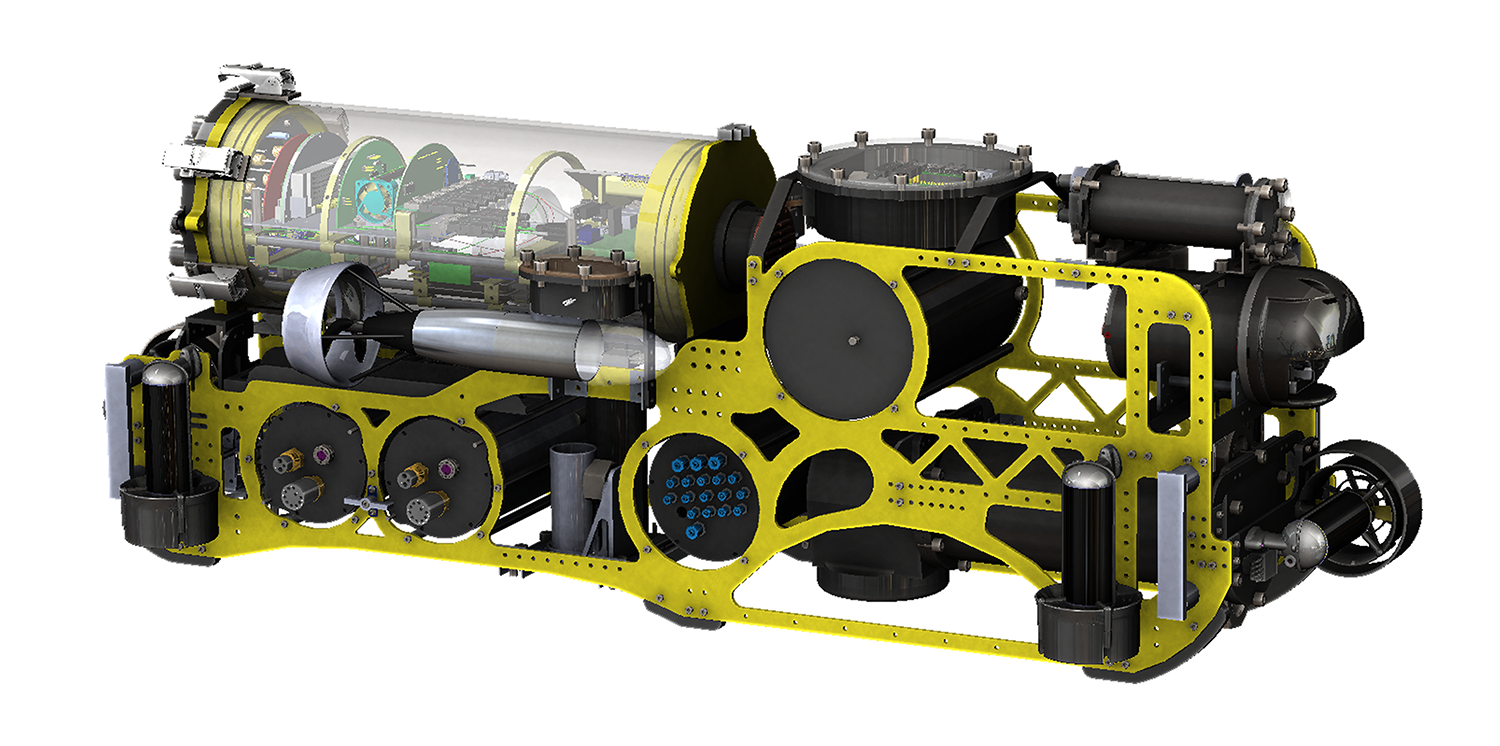
\includegraphics[width=0.5\textwidth, height=0.3\textwidth]{figs/auv.png}
  \end{figure}

  \textbf{AUV} is a robot that travels underwater without requiring input from an operator.

\end{frame}

\begin{frame}{Some applications of AUV}

  \begin{figure}[ht]
      \centering
      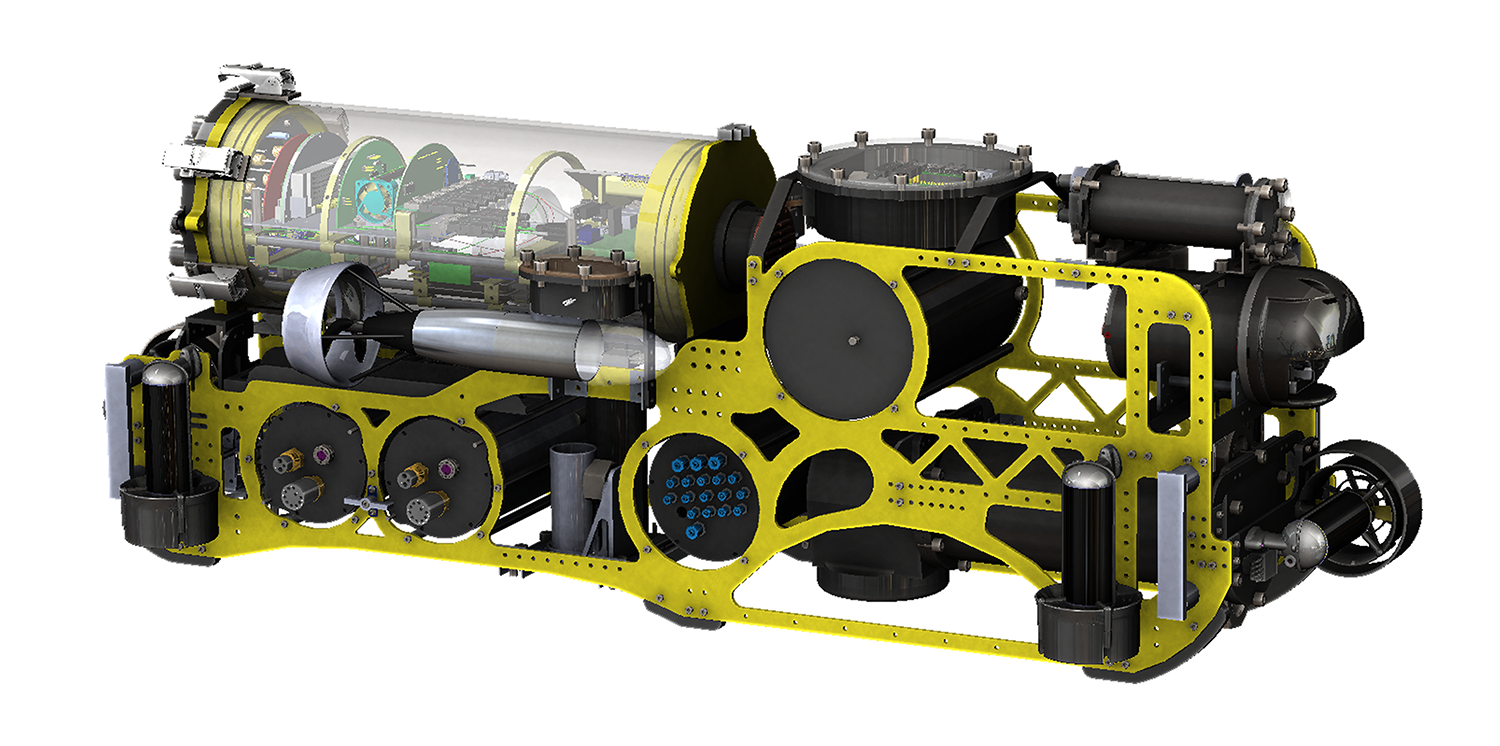
\includegraphics[width=0.5\textwidth, height=0.3\textwidth]{figs/auv.png}
  \end{figure}

  \begin{enumerate}
    \item Air crash investigation
    \item Conduct research on life of marine organisms
    \item Make detailed maps of the seafloor
  \end{enumerate}

\end{frame}

\begin{frame}{Robosub}

  \begin{figure}[ht]
      \centering
      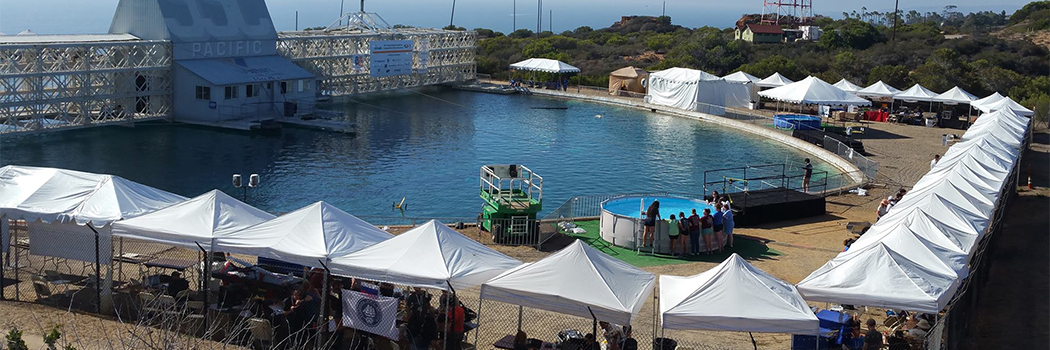
\includegraphics[width=0.5\textwidth, height=0.3\textwidth]{figs/robosub.jpg}
  \end{figure}

  \textbf{Robosub} is an international AUV competition held annually in San Diego.

\end{frame}

\begin{frame}{Visual-based tasks}

  \begin{figure}[ht]
      \centering
      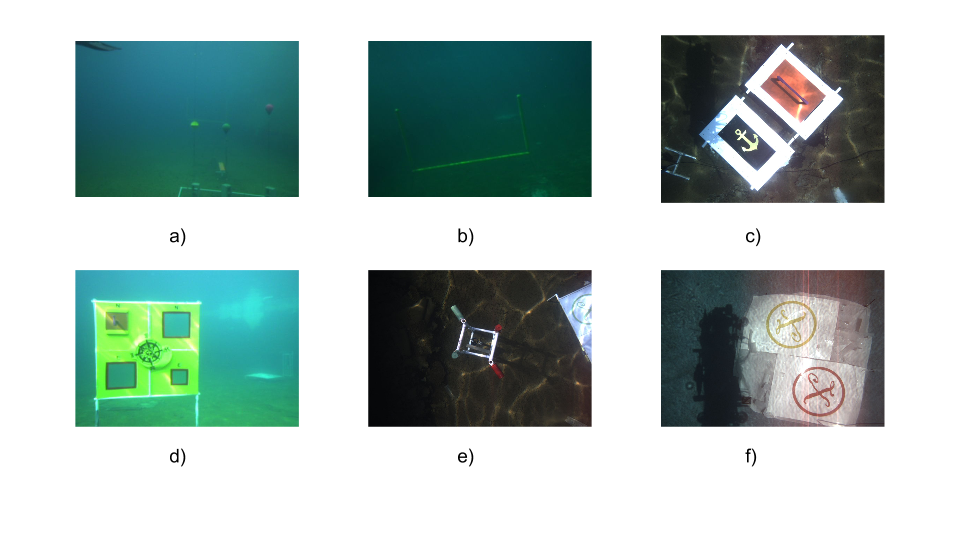
\includegraphics[width=0.6\textwidth, height=0.4\textwidth]{figs/tasks.png}
  \end{figure}

  Each AUV is required to complete a series of visual-based tasks that simulate
  the actual work of an AUV.

\end{frame}
%%%%%%%%%%%%%%%%%%%%%%%%%%%%%%%%%%%%%%%%%%%%%%%%%%%%%%%%%%%%%%%%%%%%%%%%%%%%%%%%%%%%%%%%%%%%%%%%%%%%

\begin{frame}[standout]{}
  Design a robust underwater vision framework for AUV to complete the visual tasks
  in Robosub
\end{frame}
%%%%%%%%%%%%%%%%%%%%%%%%%%%%%%%%%%%%%%%%%%%%%%%%%%%%%%%%%%%%%%%%%%%%%%%%%%%%%%%%%%%%%%%%%%%%%%%%%%%%

\section{Motivation}

\begin{frame}{1: Robust underwater object recognition}

  \begin{figure}[ht]
      \centering
      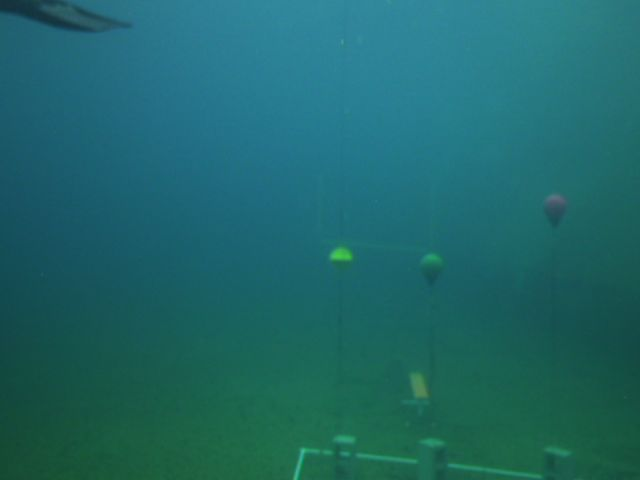
\includegraphics[width=0.5\textwidth, height=0.3\textwidth]{figs/problem1_1.png}
  \end{figure}

  Can you identify the {\color{red} \textbf{RED}} buoy ? 

\end{frame}

\begin{frame}{1: Robust underwater object recognition}

  \begin{figure}[ht]
      \centering
      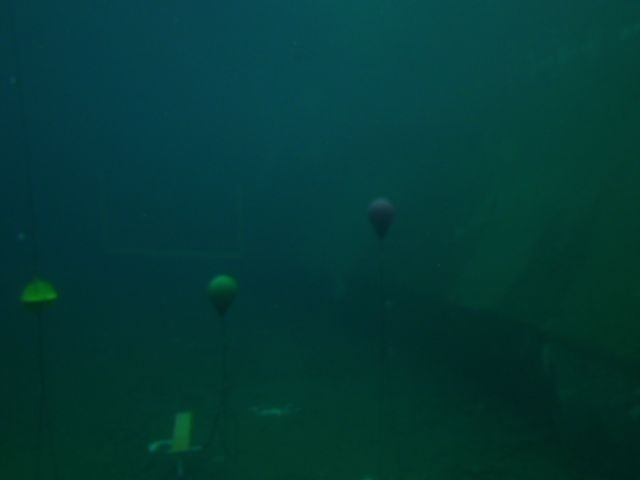
\includegraphics[width=0.5\textwidth, height=0.3\textwidth]{figs/problem1_2.jpg}
  \end{figure}

  Can you still identify the {\color{red} \textbf{RED}} buoy ? 

\end{frame}

\begin{frame}{1: Robust underwater object recognition}

    \begin{figure}
        \centering
        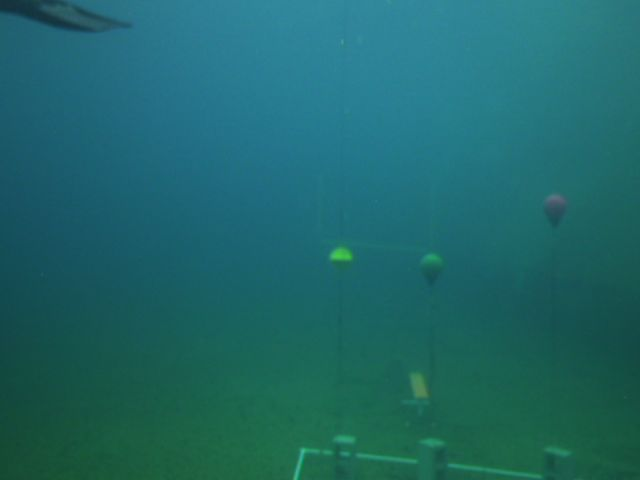
\includegraphics[width=0.4\textwidth, height=0.3\textheight]{figs/problem1_1.png}\hspace{2em}
        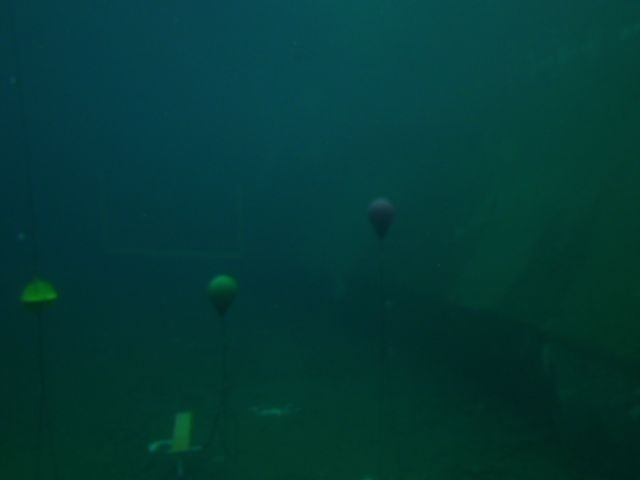
\includegraphics[width=0.4\textwidth, height=0.3\textheight]{figs/problem1_2.jpg}
    \end{figure}

  How do we \textbf{consistently} identify the object of interest under
  different conditions ?

\end{frame}

\begin{frame}{1: Robust underwater object recognition}
  \begin{figure}[ht]
      \centering
      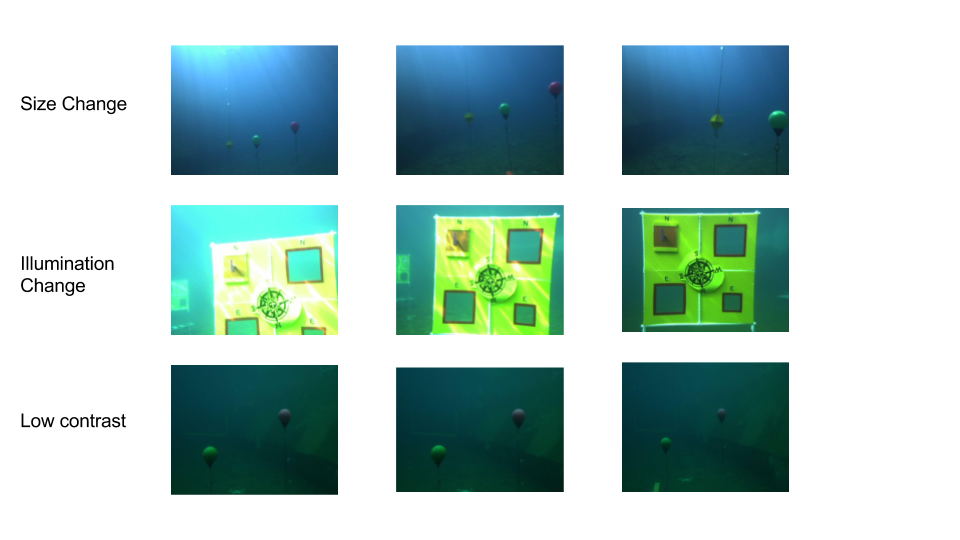
\includegraphics[width=0.9\textwidth, height=0.6\textwidth]{figs/data1.png}
  \end{figure}
\end{frame}

\begin{frame}{1: Robust underwater object recognition}
  \begin{figure}[ht]
      \centering
      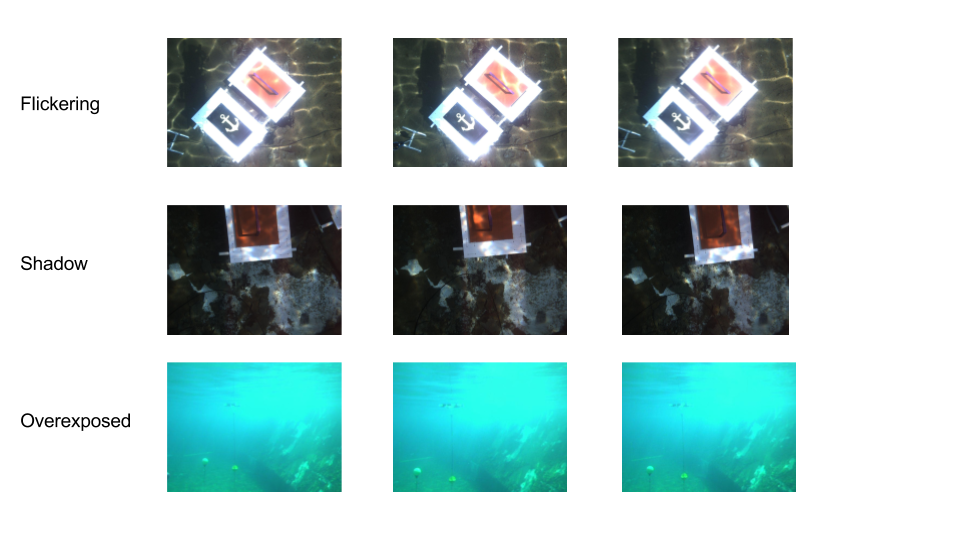
\includegraphics[width=0.9\textwidth, height=0.6\textwidth]{figs/data2.png}
  \end{figure}
\end{frame}

\begin{frame}{2: Do more with less}

    \begin{figure}[ht]
        \centering
        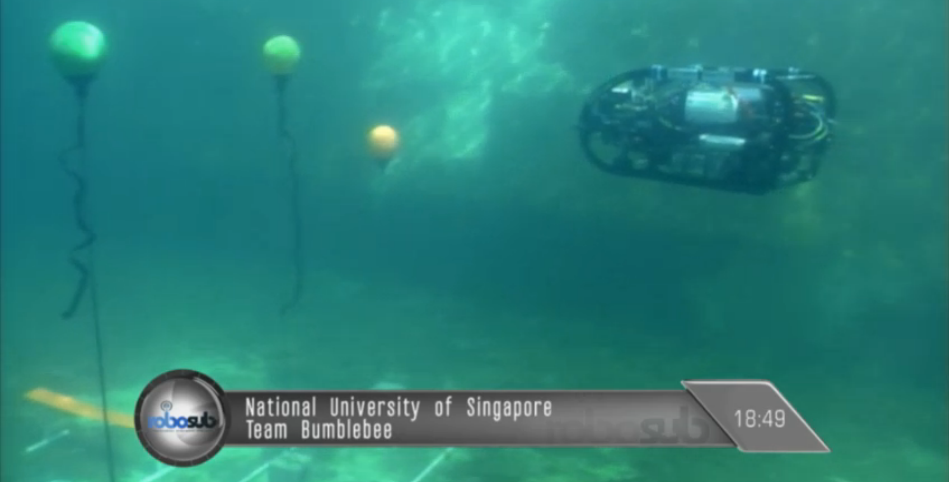
\includegraphics[width=0.4\textwidth, height=0.3\textheight]{figs/problem2_1.png}\hspace{2em}
        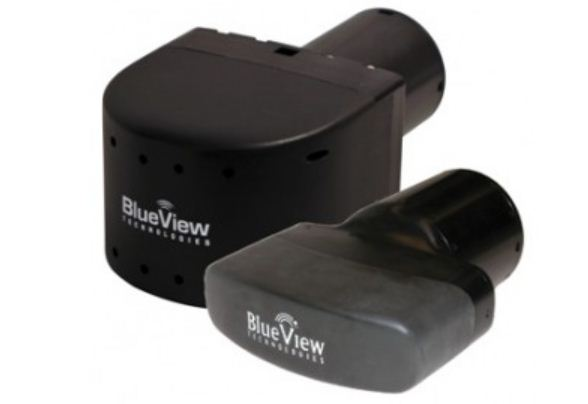
\includegraphics[width=0.4\textwidth, height=0.3\textheight]{figs/sonar.jpg}
    \end{figure}

  \begin{enumerate}
    \item Limited amount of training data because data collection is expensive
    \item Limited amount of time to complete all the designated tasks
    \item \textbf{VISUAL} only approach without other sensors such as a sonar.
  \end{enumerate}

\end{frame}

\begin{frame}{3: Taking human out of the loop}

  \begin{figure}[ht]
      \centering
      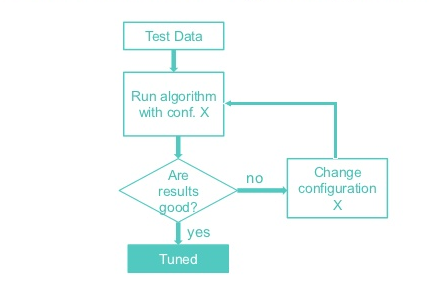
\includegraphics[width=0.6\textwidth, height=0.3\textwidth]{figs/tuning.png}
  \end{figure}

  \begin{enumerate}
    \item Spend less time on tuning the algorithms for different conditions
    \item A vision framework that is able to adapt to different situations
  \end{enumerate}

\end{frame}
%%%%%%%%%%%%%%%%%%%%%%%%%%%%%%%%%%%%%%%%%%%%%%%%%%%%%%%%%%%%%%%%%%%%%%%%%%%%%%%%%%%%%%%%%%%%%%%%%%%%

\begin{frame}[standout]{Contributions}
  \begin{enumerate}
    \item Optimal preprocessing pipeline for underwater object tracking
    \item Integrating object proposals for faster tracking
    \item Novel color spaces for feature extraction
  \end{enumerate}
\end{frame}
%%%%%%%%%%%%%%%%%%%%%%%%%%%%%%%%%%%%%%%%%%%%%%%%%%%%%%%%%%%%%%%%%%%%%%%%%%%%%%%%%%%%%%%%%%%%%%%%%%%%

\section{Preprocessing}

\begin{frame}{Color Correction}
    \begin{figure}
        \centering
        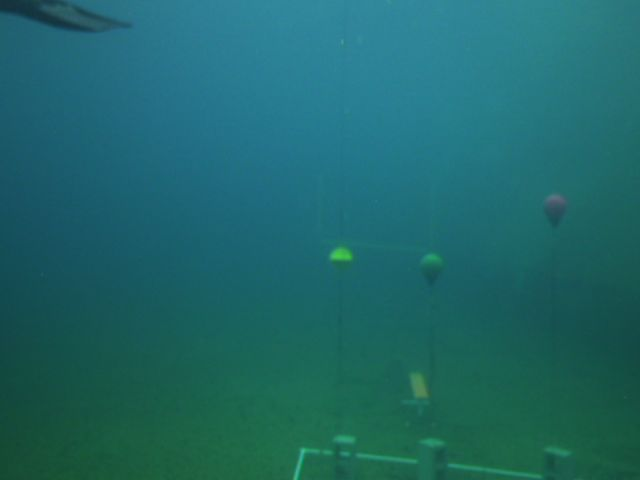
\includegraphics[width=0.4\textwidth, height=0.3\textheight]{figs/problem1_1.png}\hspace{2em}
        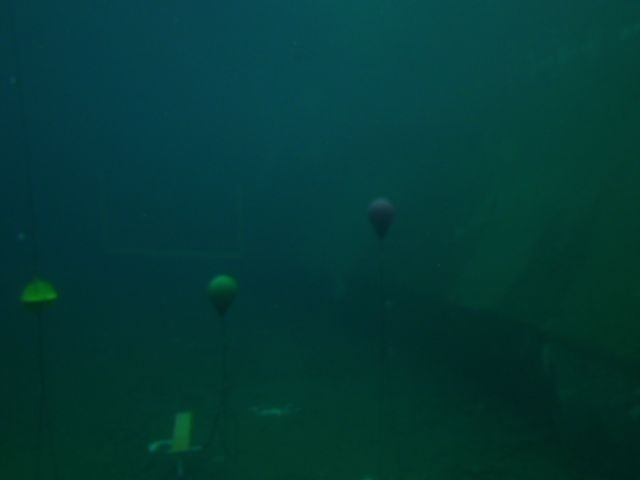
\includegraphics[width=0.4\textwidth, height=0.3\textheight]{figs/problem1_2.jpg}
    \end{figure}

    Ability to correct colour of an object under the influence of different
    light source.

\end{frame}

\begin{frame}{Color Correction: Estimate the true illuminant}

  \begin{figure}[ht]
      \centering
      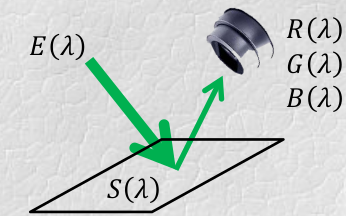
\includegraphics[width=0.6\textwidth, height=0.3\textwidth]{figs/lambertian.png}
  \end{figure}

  \begin{gather*}
    C(\lambda) = E(\lambda)S(\lambda) \\         \text{where~$C(\lambda)$:
      color signal, $E(\lambda)$: illuminance, $S(\lambda)$: reflectance}
  \end{gather*}

  \begin{enumerate}
    \item Shades of Gray
    \item Estimation using Grey Pixel
  \end{enumerate}
\end{frame}

\begin{frame}{Color Correction: Using Grey Pixel}

  \begin{figure}[ht]
      \centering
      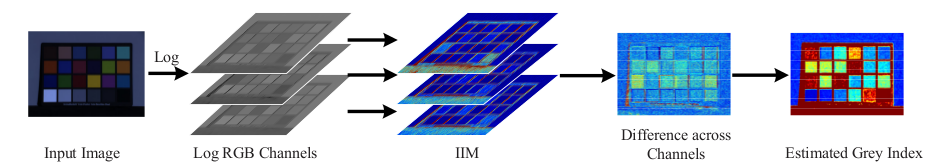
\includegraphics[width=0.6\textwidth, height=0.2\textwidth]{figs/greypixel.png}
  \end{figure}

  \begin{enumerate}
    \item With the assumption that most natural images have grey pixels under a
      white light source, identify these grey pixels
    \item Convert the image to logarithm space to remove the effect of illuminance
      \[
        I_{log}(x,y) = \log(E(x,y)) + \log(R(x,y))
      \]
    \item Find difference between the local standard deviation of 3 channels. A
      grey pixel should have approximately \textit{zero} difference.
  \end{enumerate}
\end{frame}

\begin{frame}{Color Correction: Diagonal transformation}
      The corrected image is obtained by multiplying a diagonal matrix with
      the input image
      \[
      \begin{pmatrix}
        R_c \\
        G_c \\
        B_c \\
      \end{pmatrix}
      =
      \begin{pmatrix}
        d_1 & 0 & 0 \\
        0 & d_2 & 0 \\
        0 & 0 & d_3\\
      \end{pmatrix}
      \begin{pmatrix}
        R_u \\
        G_u \\
        B_u \\
      \end{pmatrix}
      \]
\end{frame}

\begin{frame}{Color Correction: Results}

  \begin{figure}[ht]
      \centering
      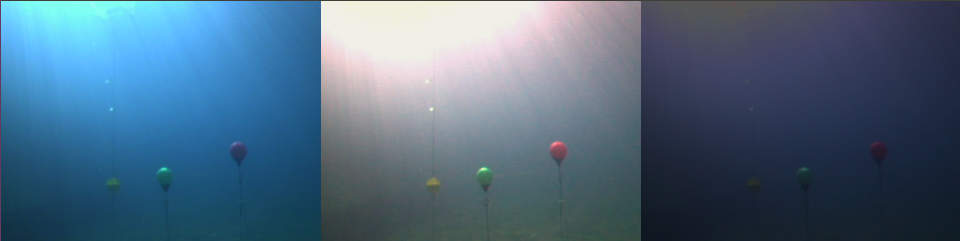
\includegraphics[width=0.6\textwidth, height=0.2\textwidth]{figs/colorcorrection.png}
      \caption{Results: a) Input Image, b) Shade of Gray, c) Grey Pixel}
  \end{figure}

  Combination of different color constancy algorithms produce the best result.

\end{frame}

\begin{frame}{Fusion-based enhancement: Overview}

  \begin{figure}[ht]
      \centering
      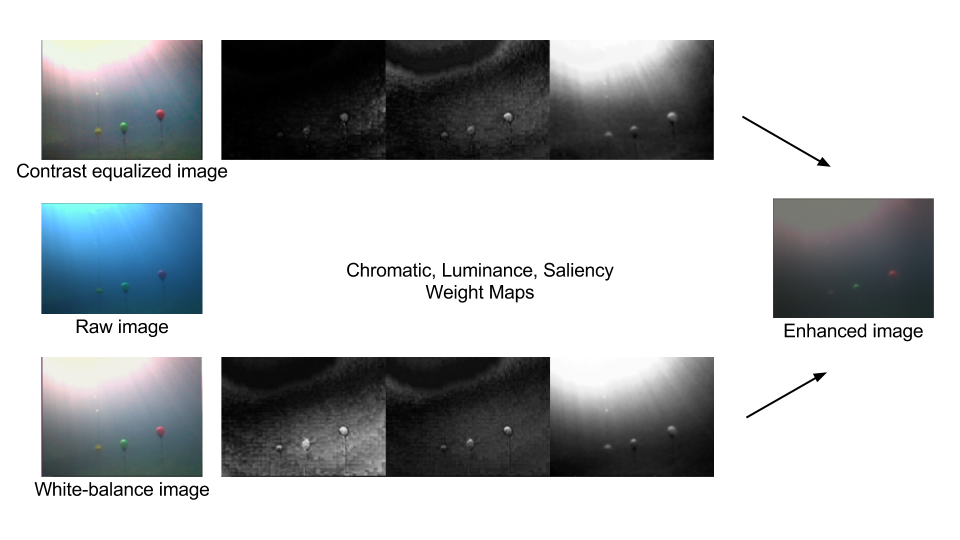
\includegraphics[width=0.9\textwidth, height=0.6\textwidth]{figs/fusion_pipeline.png}
  \end{figure}

\end{frame}

\begin{frame}{Methodology: Preprocess input}
  \begin{enumerate}
    \item Compute color corrected image as \textbf{\textit{input1}}
    \item Compute contrast enhanced \textit{input1} as \textbf{\textit{input2}}
  \end{enumerate}
\end{frame}

\begin{frame}{Methodology: Compute weight maps}

  \begin{figure}[ht]
      \centering
      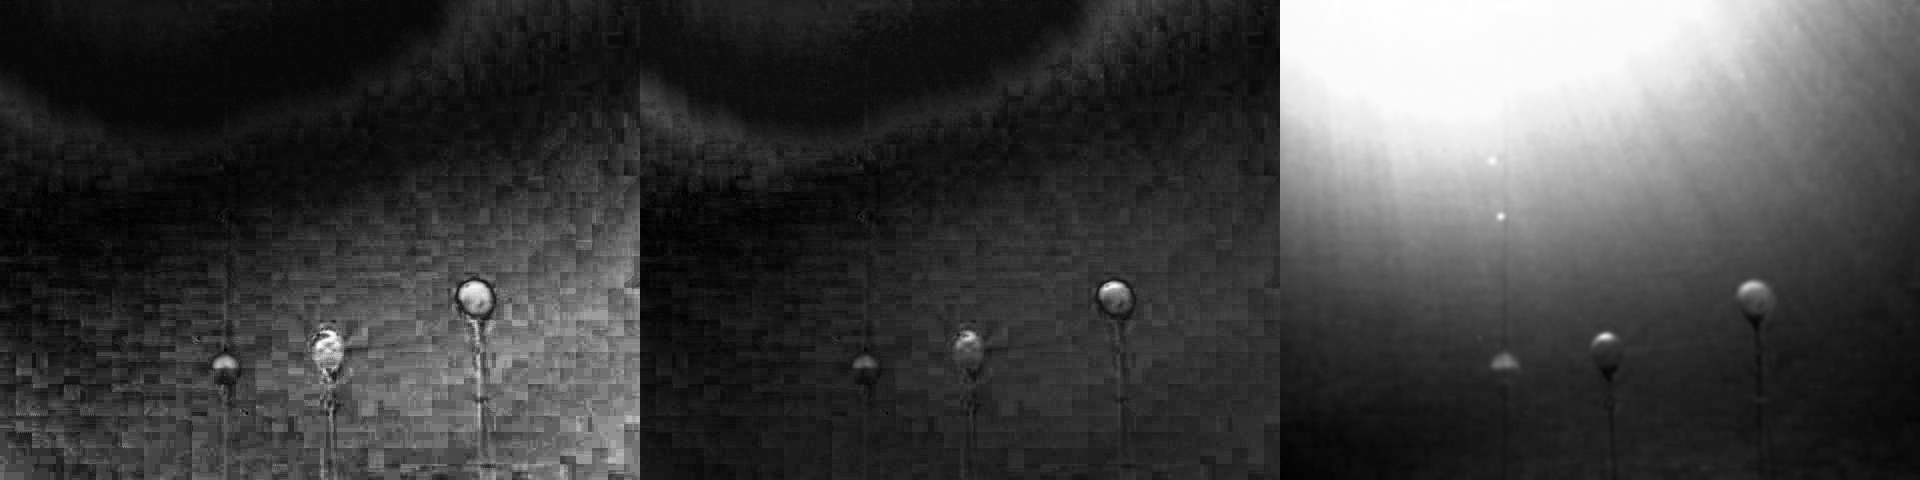
\includegraphics[width=0.5\textwidth, height=0.2\textwidth]{figs/weightmaps.png}
      \caption{Weight maps (left to right): chromatic map, luminance map,
        saliency map}
  \end{figure}

  \begin{enumerate}
    \item Compute weight maps for \textit{input1} and \textit{input2}
    \item Normalize the 2 sets of weight maps
  \end{enumerate}
\end{frame}

\begin{frame}{Methodology: Pyramid-based image fusion}

  \begin{figure}[ht]
      \centering
      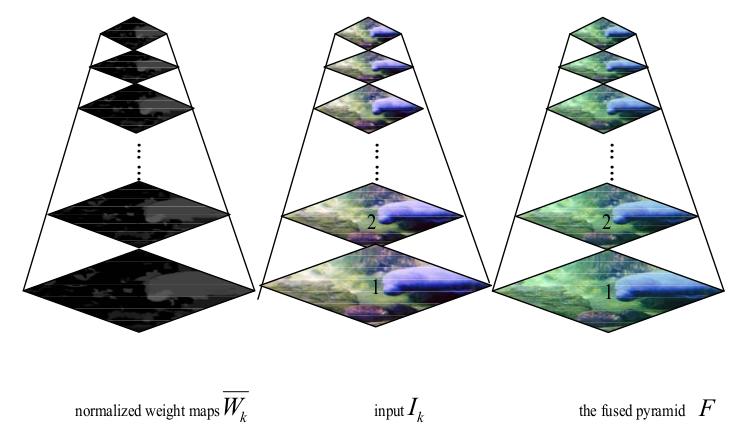
\includegraphics[width=0.8\textwidth, height=0.4\textwidth]{figs/pyramid.png}
  \end{figure}

  \begin{enumerate}
    \item Generates image pyramid for each inputs and weight maps
    \item Fuse the normalized weight maps with input  using the generated pyramids
  \end{enumerate}
\end{frame}

\begin{frame}{Image denoising: Homomorphic filter}

  \begin{figure}[ht]
      \centering
      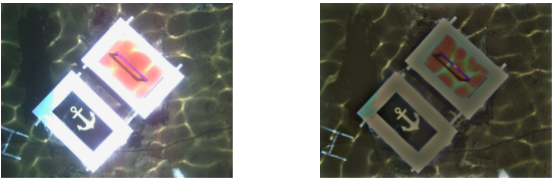
\includegraphics[width=0.6\textwidth, height=0.3\textwidth]{figs/homomorphic.png}
  \end{figure}

  \textbf{Homomorphic filter} removes multiplicative noise by applying high-pass
  filter on the image. This is the most effective way of removing the flickering
  effect from the input image.

\end{frame}

\begin{frame}{Illumination Compensation}

  \begin{figure}[ht]
      \centering
      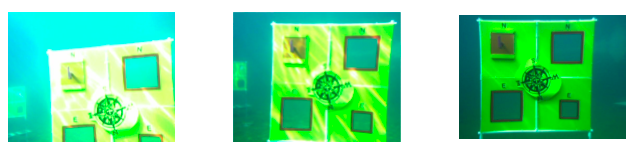
\includegraphics[width=0.8\textwidth, height=0.3\textwidth]{figs/illumcompensation.png}
  \end{figure}

  How do we account for change in illumination during the mission ?

  \begin{enumerate}
    \item Changing the camera parameters before the start of every run
    \item Use another sensor that is invariant to change in illumination i.e
      acoustic based
  \end{enumerate}
  
\end{frame}

\begin{frame}{Illumination Compensation}

  \begin{figure}[ht]
      \centering
      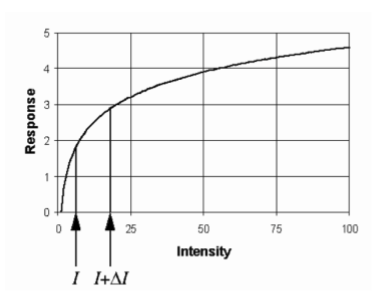
\includegraphics[width=0.6\textwidth, height=0.3\textwidth]{figs/logcurve.png}
  \end{figure}

  \[
    I'(x,y) = \frac{\log(I(x,y)) \cdot (\beta -1) + 1}{\log(\beta)}
  \]
  A logarithm curve is used to correct the camera's response based on the
  parameter $\beta$.
\end{frame}

\begin{frame}{How to determine $\beta$ ?}
  \[
    \beta' = (\beta_{max}- \beta_{min}) \cdot (N_{darkpixels} / N_{totalpixels})
    + \beta_{min}
  \]
  \begin{enumerate}
    \item Choose the range for value of $\beta$. This will determine the degree
      of enhancement allowed
    \item Choose a threshold for dark pixels. Through empirical evaluations, a
      value of \textit{0.2} is chosen
    \item Illumination compensation is only triggered when the mean intensity of
      image falls below a certain threshold.
  \end{enumerate}
\end{frame}
%%%%%%%%%%%%%%%%%%%%%%%%%%%%%%%%%%%%%%%%%%%%%%%%%%%%%%%%%%%%%%%%%%%%%%%%%%%%%%%%%%%%%%%%%%%%%%%%%%%%

\section{Object Proposals}

\begin{frame}{How it used to work: Sliding window}

  \begin{figure}[ht]
      \centering
      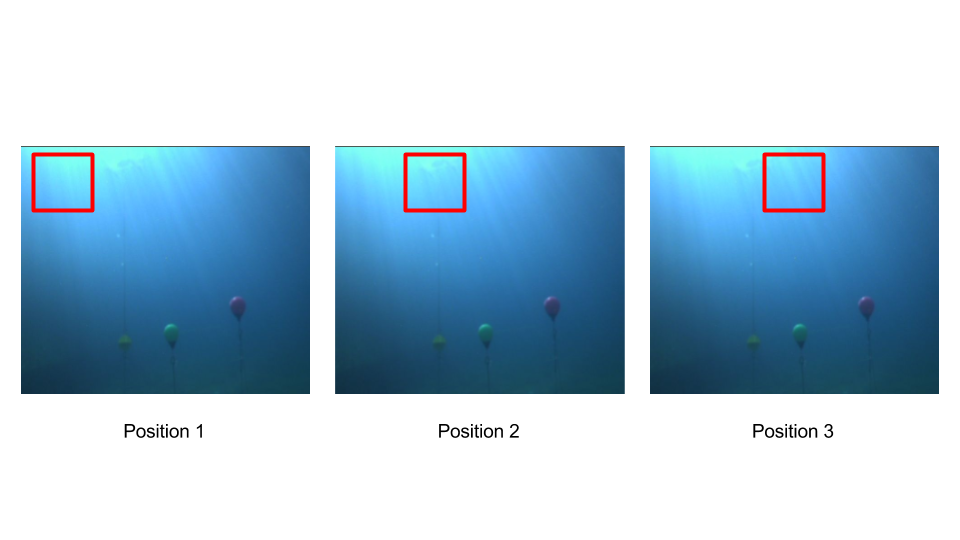
\includegraphics[width=0.7\textwidth, height=0.4\textwidth]{figs/sliding_window.png}
  \end{figure}

  Treat object recognition as \textit{classification} problem by classifying
  each window with a trained classifier. There are several \textit{drawbacks}
  with this approach:

  \begin{enumerate}
    \item Performance dependent on object classifier
    \item Computationally expensive. approximately $10^6$ evaluations per image
  \end{enumerate}
\end{frame}

\begin{frame}{Object proposal}

  \begin{figure}[ht]
      \centering
      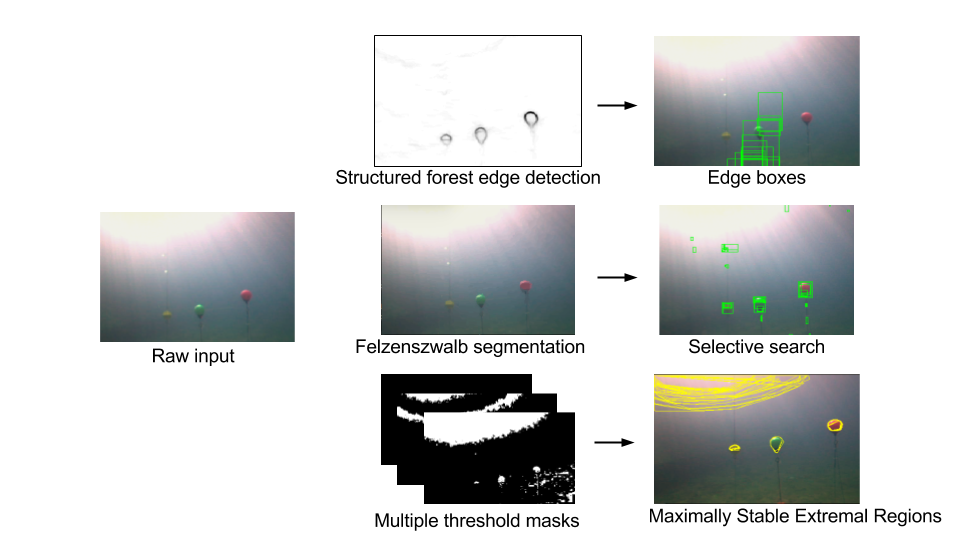
\includegraphics[width=0.8\textwidth, height=0.4\textwidth]{figs/proposals_results.png}
  \end{figure}

  \begin{enumerate}
    \item Given an input image, generates a set of windows that has high
      \textit{likelihood} of containing an object.
    \item Definition of \textbf{\textit{objectness}} depends on what algorithms are used
  \end{enumerate}
\end{frame}

\begin{frame}{Role of object proposals}

  \begin{enumerate}
    \item A more general object detector using cues like edges and color
    \item Prevent false negatives because of strict object classifiers
  \end{enumerate}
\end{frame}

\begin{frame}{1. Superpixel-based search}

  \begin{figure}[ht]
      \centering
      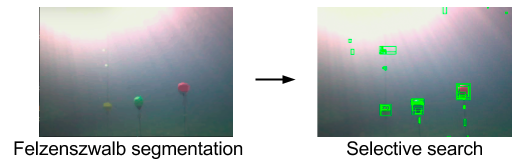
\includegraphics[width=0.8\textwidth, height=0.4\textwidth]{figs/selectivesearch.png}
  \end{figure}

  \begin{enumerate}
    \item Superpixel segmentation by grouping pixels with similar colour
    \item Hierarchical grouping of similar segments
  \end{enumerate}
\end{frame}

\begin{frame}{2. MSER (Maximally Stable Extremal Regions)}

  \begin{figure}[ht]
      \centering
      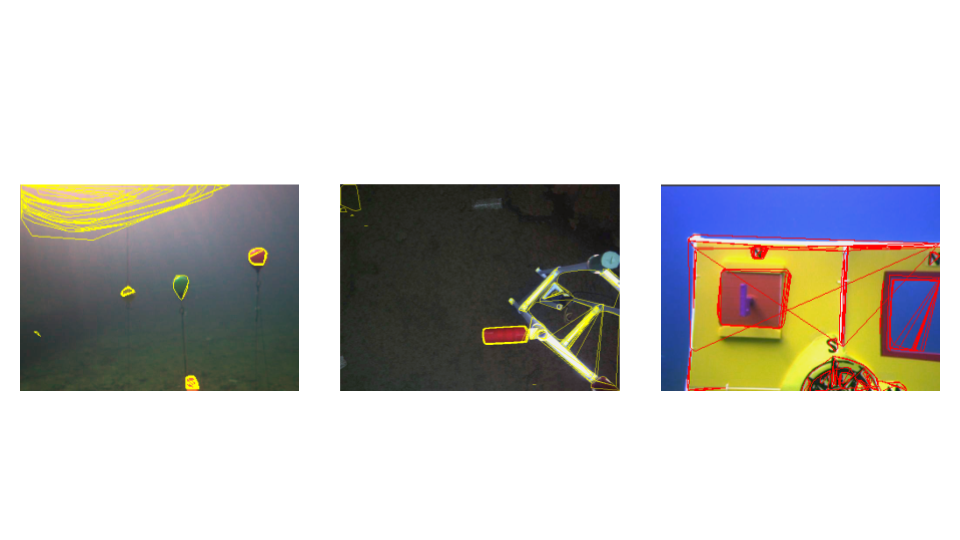
\includegraphics[width=0.8\textwidth, height=0.5\textwidth]{figs/mserproposal.png}
  \end{figure}

  Detects regions that remain stable over different thresholds applied
  on the input image. Multiple colour spaces are used in order to generate more
  segments.
\end{frame}

\begin{frame}{2. MSER (Maximally Stable Extremal Regions)}

  \begin{figure}[ht]
      \centering
      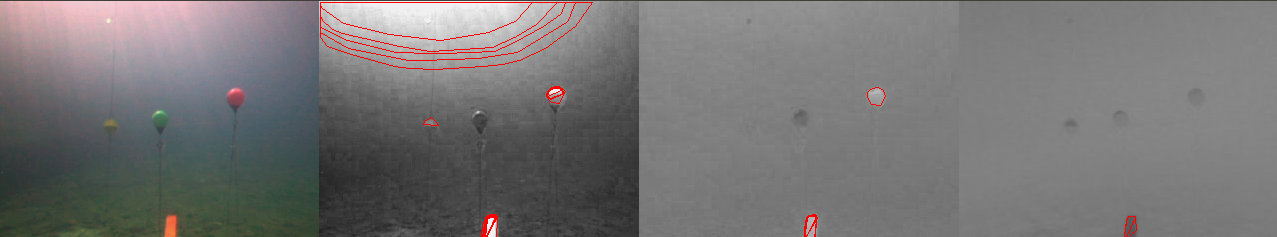
\includegraphics[width=0.7\textwidth, height=0.3\textwidth]{figs/msermix.png}
  \end{figure}

  Different colour spaces are suitable for different objects. Thus, combination
  of different colour spaces will increase the number of candidate windows.

\end{frame}
%%%%%%%%%%%%%%%%%%%%%%%%%%%%%%%%%%%%%%%%%%%%%%%%%%%%%%%%%%%%%%%%%%%%%%%%%%%%%%%%%%%%%%%%%%%%%%%%%%%%

\section{Feature Design}

\begin{frame}{Requirements}
  To achieve a consistent object tracking under different sets of challenges,
  the features used for training needs to achieve certain degree of invariance.
  \begin{enumerate}
    \item Illumination invariance
    \item Scale \& rotation invariance
  \end{enumerate}
\end{frame}

\begin{frame}{Color descriptors}

  \begin{figure}[ht]
      \centering
      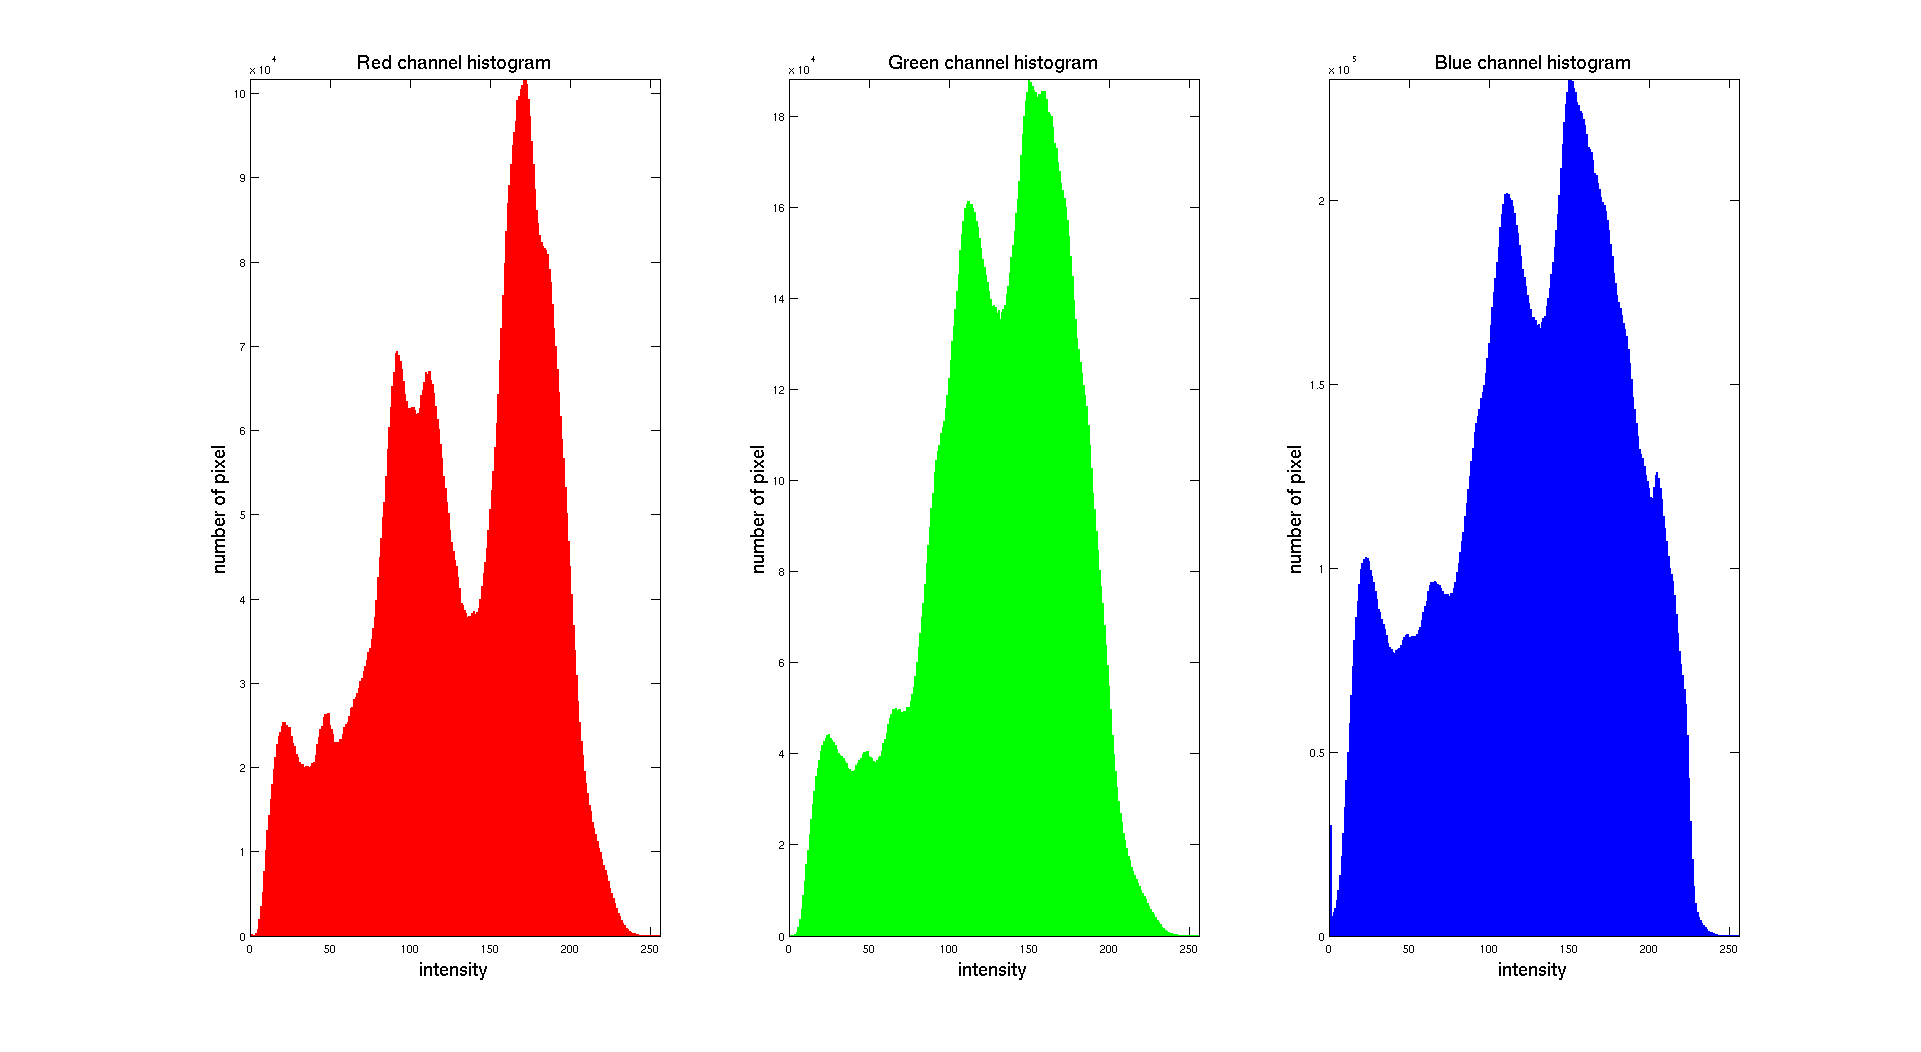
\includegraphics[width=0.6\textwidth, height=0.3\textwidth]{figs/colorhistogram.png}
  \end{figure}

  Color features are chosen as the primary features because of:
  \begin{enumerate}
    \item Highly-invariant to scale and rotation
    \item Highly discriminative as different objects possess different colors
  \end{enumerate}

\end{frame}

\begin{frame}{Caveat 1: Sensitive to illumination}

  \begin{figure}[ht]
      \centering
      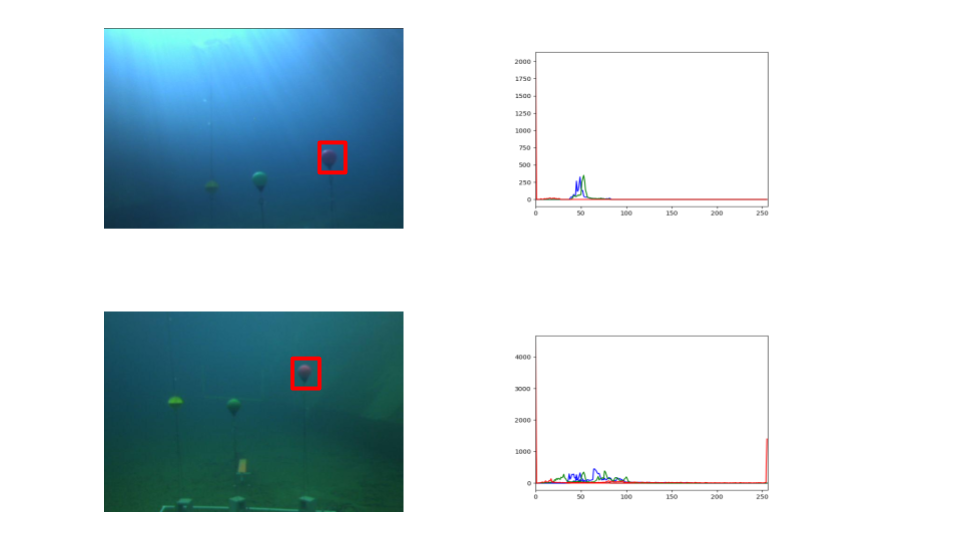
\includegraphics[width=0.6\textwidth, height=0.3\textwidth]{figs/illumsensitive.png}
  \end{figure}

  \begin{enumerate}
    \item Perform color correction to input image before feature extraction
    \item Explore different color spaces that are illumination-invariant
  \end{enumerate}

\end{frame}

\begin{frame}[standout]{}
  Changing color space
\end{frame}

\begin{frame}{rg chromacity}

  \begin{figure}[ht]
      \centering
      
\includegraphics[width=0.5\textwidth, height=0.3\textwidth]{figs/rg.png}
  \end{figure}

  Removes influence of luminance through normalization 
  \[
    r = \frac{R}{R + G + B}, g = \frac{G}{R + G + B}, b = \frac{B}{R + G + B}
  \]
\end{frame}

\begin{frame}{Opponent color space}

  Provides small amount of illumination invariance while maintaning
  discriminative power.
  \[
  \begin{aligned}
    O1 = \frac{R - G}{\sqrt{2}}, O2 = \frac{R + G - 2B}{\sqrt{6}}, O3 = \frac{R +
      G + B}{\sqrt{3}} \\
    W_{o1} = \frac{O1}{O3}, W_{o2} = \frac{O2}{O3}
  \end{aligned}
  \]
\end{frame}

\begin{frame}{Log color ratio}

  Provides complete illumination invariance.
  \[
    L1 = \log{\frac{R}{B}}, L2 = \log{\frac{R}{B}}, L3 = \log{\frac{G}{B}}
  \]
\end{frame}

\begin{frame}{Caveat 2: Insenstive to shape}

  Concatenating shape descriptor with color descriptor. Shape descriptors
  extracted include:

  \begin{enumerate}
    \item Inner shape context
    \item Elliptic Fourier descriptor
    \item Zernike moment
    \item Hu moment
  \end{enumerate}

\end{frame}

%%%%%%%%%%%%%%%%%%%%%%%%%%%%%%%%%%%%%%%%%%%%%%%%%%%%%%%%%%%%%%%%%%%%%%%%%%%%%%%%%%%%%%%%%%%%%%%%%%%%

\section{Object Tracking}

\begin{frame}{Tracking by detection}

  \begin{figure}[ht]
      \centering
      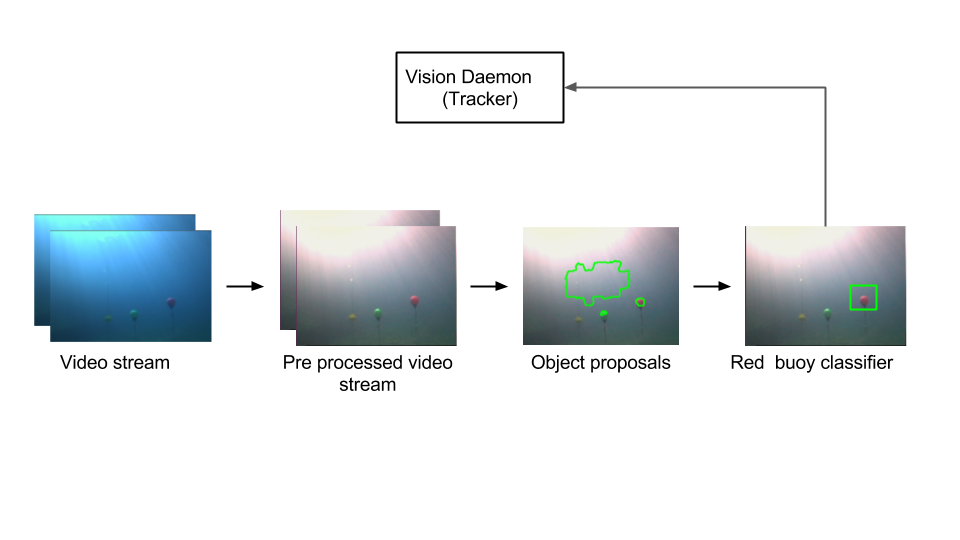
\includegraphics[width=0.8\textwidth, height=0.4\textwidth]{figs/tracker.png}
  \end{figure}

  \begin{enumerate}
    \item Detection is performed on every single incoming frame
    \item Tracker is reinitialized after losing track for at least 10 frames
  \end{enumerate}
\end{frame}

\begin{frame}{Scoring mechanism}
  A final score is calculated for each candidate window generated by object
  proposal algorithm.
  \[
    Score_{final} = (1 - \alpha) Score_{classification} + \alpha Score_{prior}
  \]
  The weighted combination of \textit{classification score} and \textit{prior
    score} is used to calculate the final score.
\end{frame}

\begin{frame}{Prior knowledge: Using Map}

  \begin{figure}[ht]
      \centering
      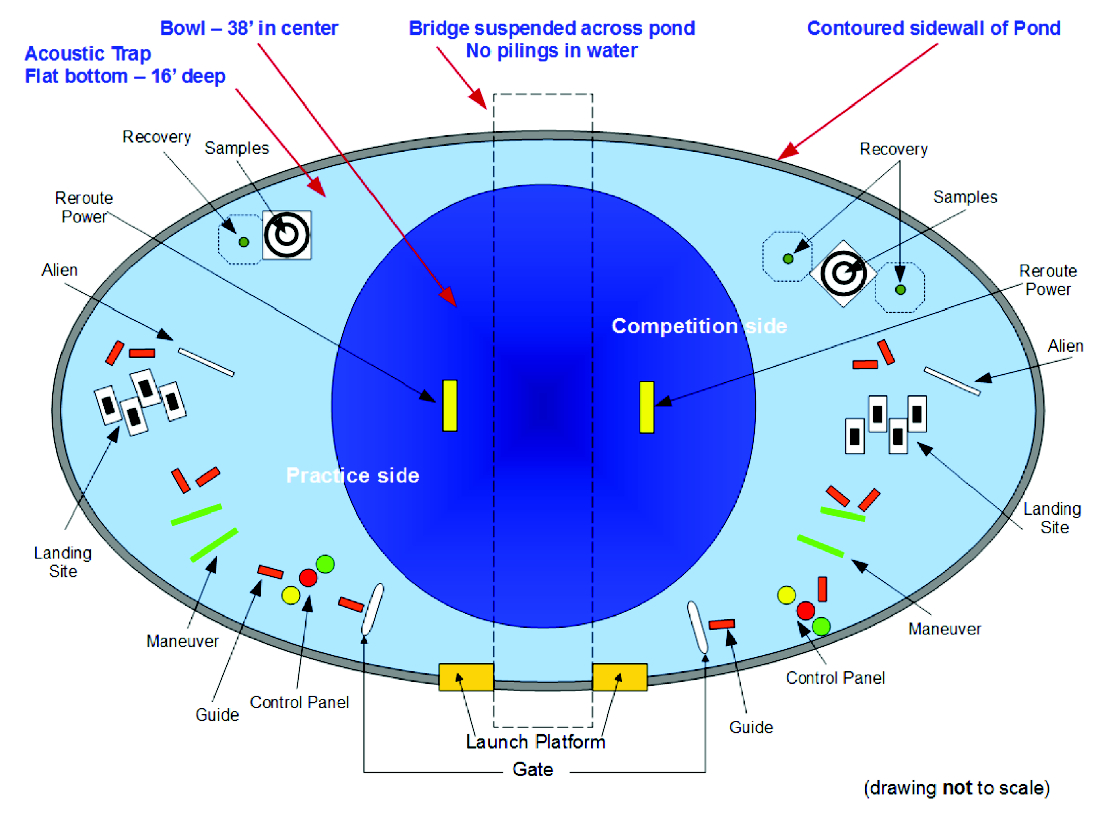
\includegraphics[width=0.8\textwidth, height=0.4\textwidth]{figs/map.jpg}
  \end{figure}

  Based on the current location of AUV, a confidence map can be generated based
  on the given layout. This extra information can help to eliminate some false
  positives.
\end{frame}

\begin{frame}{Prior knowledge: Geometric constraint}

  \begin{figure}[ht]
      \centering
      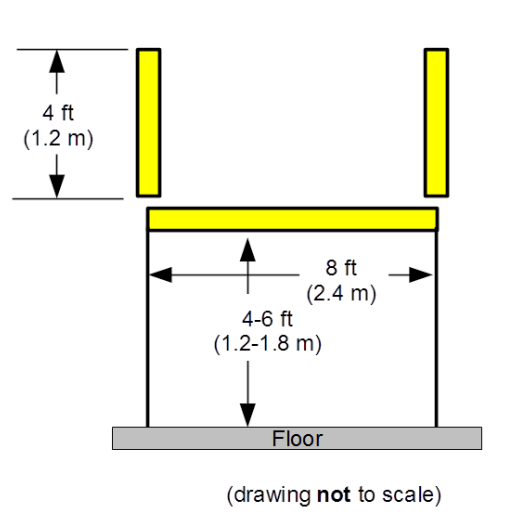
\includegraphics[width=0.6\textwidth, height=0.4\textwidth]{figs/geometric.png}
  \end{figure}

  Each object candidate will also be ranked according to \textit{geometric
    properties} given by the event organizer to achieve higher accuracy of detection.

\end{frame}

\section{Experimental results}

\begin{frame}{Results}

\begin{table}[H]
\resizebox{.8\textwidth}{!}{
\centering
\begin{tabular}{|l|l|l|l|}
\hline
Trackers                           & Accuracy & Robustness & Speed (FPS) \\ \hline
Baseline                           & 0.21     & 7.23       & 200   \\ \hline
Baseline + preprocessing           & 0.34     & 6.11       & 50    \\ \hline
Baseline + preprocessing +  automl & 0.53     & 2.53       & 50    \\ \hline
MOSSE                              & 0.30     & 8.10       & 100   \\ \hline
KCF                                & 0.35     & 4.91       & 70    \\ \hline
EBT (Edge Box Tracker)             & 0.41     & 3.11       & 43    \\ \hline
\end{tabular}
}
\end{table}

\end{frame}

\begin{frame}[standout]{}
  Q \& A
\end{frame}
%%%%%%%%%%%%%%%%%%%%%%%%%%%%%%%%%%%%%%%%%%%%%%%%%%%%%%%%%%%%%%%%%%%%%%%%%%%%%%%%%%%%%%%%%%%%%%%%%%%%
\end{document}